\section{简介}

深度神经网络(DNN)是非常强大的机器学习模型,在诸如语音识别 \cite{hinton12,dahl12b} 和视觉对象识别 \cite{kriz12,ciresan12,lecun98,le12} 等困难问题上取得了出色的性能。DNN很强大,因为它可以在适当数量的步骤内执行任意的并行计算。强大DNN的一个令人惊讶的例子是他们只使用2个隐藏层就能够排序$N$个 \!\!\!\!\quad $N$位数的能力\cite{razborov}。因此,虽然神经网络与常规统计模型相关,但他们能学习一个复杂的计算。
此外当标记的训练集合具有足够的信息来指定网络的参数时,可以利用监督反向传播来训练大型的DNN。因此,如果存在实现良好结果的大型DNN的参数设置(例如,由于人类可以非常快速地解决任务),则监督反向传播将找到这些参数并解决问题。

尽管DNN具有灵活性和强大的功能,但DNN只能应用于输入和输出都用固定维数的向量编码的问题。这存在一个明显的限制,因为许多重要的问题最好用长度不为已知的先验的序列表示。例如,语音识别和机器翻译是序列问题。同样,问题回答也可以被看作是将表示问题的单词序列映射到表示答案的单词序列。因此学习将序列映射到序列且不受领域限制的方法将是非常有用的。

序列对DNN提出了挑战,因为DNN要求输入和输出的维数是已知的和固定的。
%%And
%%while Recurrent Neural Networks (RNNs) are natural candidates for this
%%task, they assume that there is a one-to-one correspondence between
%%the timesteps in the input and the output sequences, which is an
%%unrealistic assumption for most problems.
在本文中,我们表明长短期记忆(LSTM)的结构\cite{hochreiter97}的应用可以解决一般序列到序列问题。该想法是使用一个LSTM读取输入序列,一次一个时间步长,来获得一个大的固定维度向量表示,然后使用另一个LSTM从该向量提取输出序列(图~\ref{fig:translation-model2})。第二个LSTM除了它是以输入序列为条件,本质上是一个循环神经网络语言模型\cite{rumelhart1986learning,mikolov2010recurrent,sundermeyer12}。LSTM能够成功学习具有长时间依赖性数据的能力使得它成为这种应用的自然选择,因为输入及其相应输出之间存在相当大的时间滞后(图~\ref{fig:translation-model2})。

业界已经有许多相关的尝试,使用神经网络来解决一般的序列学习问题。我们的方法与Kalchbrenner和Blunsom\cite{kal13}的方法密切相关,他们是第一个将整个输入句子映射到向量的人,并且与Cho等人\cite{cho14}方法非常相似,尽管后者仅仅用于由一个基于短语的系统生成的rescoring hypotheses。Graves\cite{graves13c}引入了一种新的可区分的注意力机制,允许神经网络专注于输入的不同部分,这个想法的一个优雅的变体成功地应用于Bahdanau等人\cite{bog14}的机器翻译。连接序列分类是使用神经网络来将序列映射到序列的另一种流行的技术,尽管它假设输入和输出之间是单调对齐的\cite{graves1}。


%% There have been a number of related attempts to address the general
%% sequence to sequence learning problem with neural networks.  The
%% Connectionist Sequence Classification technique uses a simple
%% HMM-transducer that assumes a monotonic alignment between the inputs
%% and the outputs \cite{graves1,graves2}.  More recently, Graves
%% \cite{graves13c} introduced a novel differentiable attention mechanism
%% that allows neural networks to sequentially focus on different parts
%% of the input, and an elegant variant of this idea was successfully
%% applied to machine translation by Bahdanau et al.~\cite{bog14}.  Our
%% approach is inspired by Kalchbrenner and Blunsom \cite{kal13} who were
%% the first to map the entire input sentence to vector, and is very similar
%% to Cho et al.~\cite{cho14} (although the model in this paper was
%% developed in parallel to Cho et al.~\cite{cho14}).  We will discuss
%% the relationship between the various approaches in section
%% \ref{sec:rel_work}.

\begin{figure}[h]
\centering 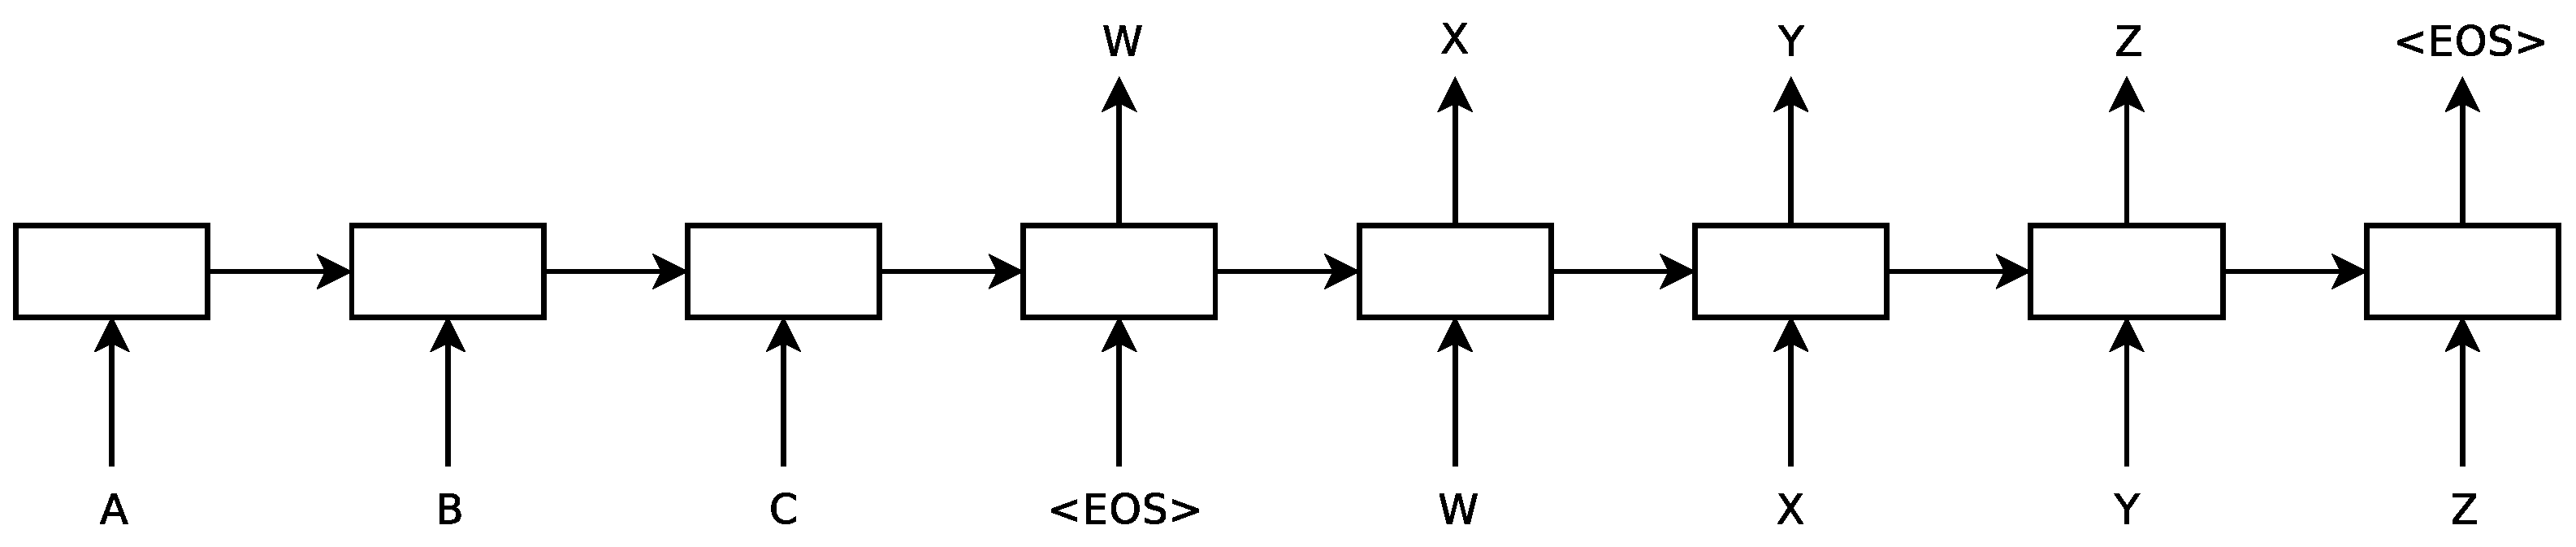
\includegraphics[width=0.9\textwidth]{Diagram1.eps}
\caption{\small 我们的模型读取输入句子“ABC”,并产生“WXYZ”作为输出句子。 该模型在输出句尾标记之后停止进行预测。 请注意,LSTM反向读取输入句子,因为这样做会在数据中引入许多短期依赖性,使得优化问题更容易。 }
\label{fig:translation-model2}
\end{figure}

这项工作的主要结果如下。在WMT'14将英语翻译成法语的任务中,我们通过使用简单的从左到右的束搜索解码直接从5个深LSTM的集合(每个具有380M个参数)中提取翻译,获得{\bf 34.81}的BLEU得分。这是迄今为止通过使用大型神经网络直接翻译所获得的最佳结果。为了比较,该数据集上的SMT基线的BLEU得分为33.30\cite{wmt14_en_fr}。通过LSTM实现的34.81 BLEU分数,词汇为80k字,所以当参考翻译包含这80k字以外的单词时,分数将被惩罚。这个结果表明比基于成熟短语的SMT系统表现更好的相对未优化的神经网络结构还具有很大的改进空间。

最后我们使用LSTM重新计算相同任务的SMT基准的1000个公开最好的列表得分\cite{wmt14_en_fr}。通过这样做,我们获得了36.5的BLEU得分,这提高了基线3.2个BLEU点,并接近以前发表过的最先进的水平(这是37.0\cite{durrani-EtAl:2014:W14-33})。

令人惊讶的是,LSTM没有遭受长句子的困扰,尽管其他研究者用相关的模型的经验表明可能会受到长句子的困扰\cite{curse}。我们能够在长句子上做得很好是因为我们颠倒了输入语句中的单词顺序,而不颠倒训练和测试集中的输出句子。通过这样做,我们引入了许多短期依赖,使优化问题更简单(见第\ref{sec:model}和\ref{sec:rev_rev}节)。因此,随机梯度下降(SGD)可以学习对长句没有问题的LSTM。在源句子中逆转单词的顺序这个技巧是这项工作的关键技术贡献之一。

LSTM的一个有用的属性是它可以学习将可变长度的输入语句映射成固定维度的向量表示。鉴于翻译往往是源语句的释义,翻译目标鼓励LSTM捕捉到其意义的句子表示,因为具有类似意义的句子彼此接近,而不同的句子意义将是远的。一个定性的评价支持表明我们的模型懂得词序,对于主动和被动语态是保持不变的。
